\section{Simulations}\label{sec:simulation}
We have conducted MATLAB simulations of different robotic systems using Simulink to compare the performance of the model-free with classical ones under different modeling inaccuracies, while holding the other robot parameters constant. Eventually we have also carried out trials in which the required theorem assumptions on the dynamics were not fully satisfied to test the limits of the reduced approach. The structure of all the control blocks for the model-free method follows the basic scheme reported in Figure~\ref{fig:simulink}.
%%% WRITE OBSTACLE POSE, DEFINE ROBOT ETC ETC
\begin{figure}[h]
    \centering
    \includegraphics[width=10cm]{../figures/schema.pdf}
    \caption{Control block structure of our model-free approach implementation. The robotic system \eqref{eq:dynamic model} outputs the pose and velocities, only the former takes a role in the safe velocity generation while the latter are used to track it.}
    \label{fig:simulink}
\end{figure}
\\
The classical approach does not implement the safe velocity tracker because the input is directly given to the robot since we are not using any approximation of the dynamics.

\subsection{Double Integrator}
As the simplest instantiation of \eqref{eq:dynamic model}, let us consider a point robot which dynamics can be modeled by: 
\begin{equation}
    \Mm\ddot{\qv} = \Bm\uv
\end{equation}
where $\qv \in \mathbb{R}^2$ represents the planar position (m) of the robot, $\uv \in \mathbb{R}^2$, $\Bm=\boldsymbol{I_2}$ and $\Mm = \mbox{diag}\left\{m, m\right\}$.
%A possible unsafe tracking controller which allows the robot to go from $\qv_{start}$ to $\qv_{goal}$ without taking into account the obstacles is given by :
We want to solve the problem of guiding the system from $\qv_{start}$ to $\qv_{goal}$ while avoiding circular obstacles, therefore reimaining in the safe region.
%, firstly,  in a model-free fashion and, then, in the classical full-model based approach.
% We work with multiple obstacles with  different dimensions.
% The first simulation 
% \textbf{Model-free Approach}:
\subsubsection{Model-free}
A solution which allows to navigate the system from $\qv_{start}$ to $\qv_{goal}$ using only a proportional gain and without taking into account the obstacles consists in realizing the desired velocity $\dot{\qv}_{nominal}$:   
\begin{equation}
    \dot{\qv}_{nominal}=-K_P(\qv - \qv_{goal}),\,K_p\in\mathbb{R}_{>0}.
\end{equation}
 We can avoid an obstacle of radius $R$ centered at $\qv_O$ by defining $d = \lVert \qv-\qv_O \rVert$ and the CBF:
\begin{equation}
h(\qv)=d-R
\end{equation}
% with gradient $\nabla h(\qv) = (\qv-\qv_O)/d = \nv_0$. 
% Then, we modify $\dot{\qv}_{nominal}$ in a minimally invasive fashion by solving the optimization problem \eqref{eq:optprob} attaining the safe velocity $\dot{\qv}_{safe}$.
At this point there are different solutions to track the safe velocity $\dot{\qv}_{safe}$. We started with Simulation 1 using controller \eqref{eq:mf controller}, to move the robot at rest from $\qv_{start}=(0,0)^T$ to $\qv_{goal}=(4,-1)^T$ avoiding the obstacles $\qv_{O1}=(1.5,0)^T$, $\qv_{O2}=(3,-1.5)^T$ of radius $R=0.75$ with gains $K_P = 0.2,~K_D=1$ [s$^{-1}$]. Moreover, setting also $m=1$~[Kg], we have been able to reproduce exactly the simulation proposed in \cite{mfcbf} varying $\alpha$ (Figure~\ref{fig:sim1map}).

\begin{figure}[h]
    \centering
    \includegraphics[scale=0.5]{../figures/sim1map.pdf}
    \caption{Simulation 1: Evolution of the state $\qv$ over the environment for the different values of parameter $\alpha$.}
    \label{fig:sim1map}
\end{figure}

% m=1 tutto come loro, m=15 sbanda senza "disturbo", m=15 con disturbo + 2 sim con cbf normale usando quella di venditelli
% \begin{align}
%     &\argmin_{\dot{\qv}_{safe} \in \mathbb{R}^2} \,\,(\dot{\qv}_{safe}-\dot{\qv}_{goal})^T(\dot{\qv}_{safe}-\dot{\qv}_{goal}) \notag\\
%     &\mathrm{s.t} \,\,\, \nv_0^T \dot{\qv}_{safe}\geq -\alpha(d-R)
% \end{align}
% By defining $\xv = \dot{\qv},~\xv_{safe}=\dot{\qv}_{safe}$, the safe velocity tracking controller $\uv = K_d (\xv - \xv_{goal}), K_d \in \mathbb{R}_{>0} $ guarantees the asynptotic convergence of $\xv$ to $\xv_{safe}$. \\
% \textbf{Remark 1.} The double integrator system avoids the obstacles, although the second-order dynamics was not directly taken into account during the CBF and control design. It follows that the CBF has relative degree $1$ with respect to $y = \qv$ if we are assuming to control the robot in velocities i.e. $\dot{\qv}=\vv$. \\
% \textbf{Remark 2.} The condition for safety consists in picking a small enough $\alpha$-value (e.g $0.1$,$0.2$).

% bisogna scrivere che non può essere usata come cbf la stessa perché il grado relativo deve essere 1, l'input apparire quando si deriva


% 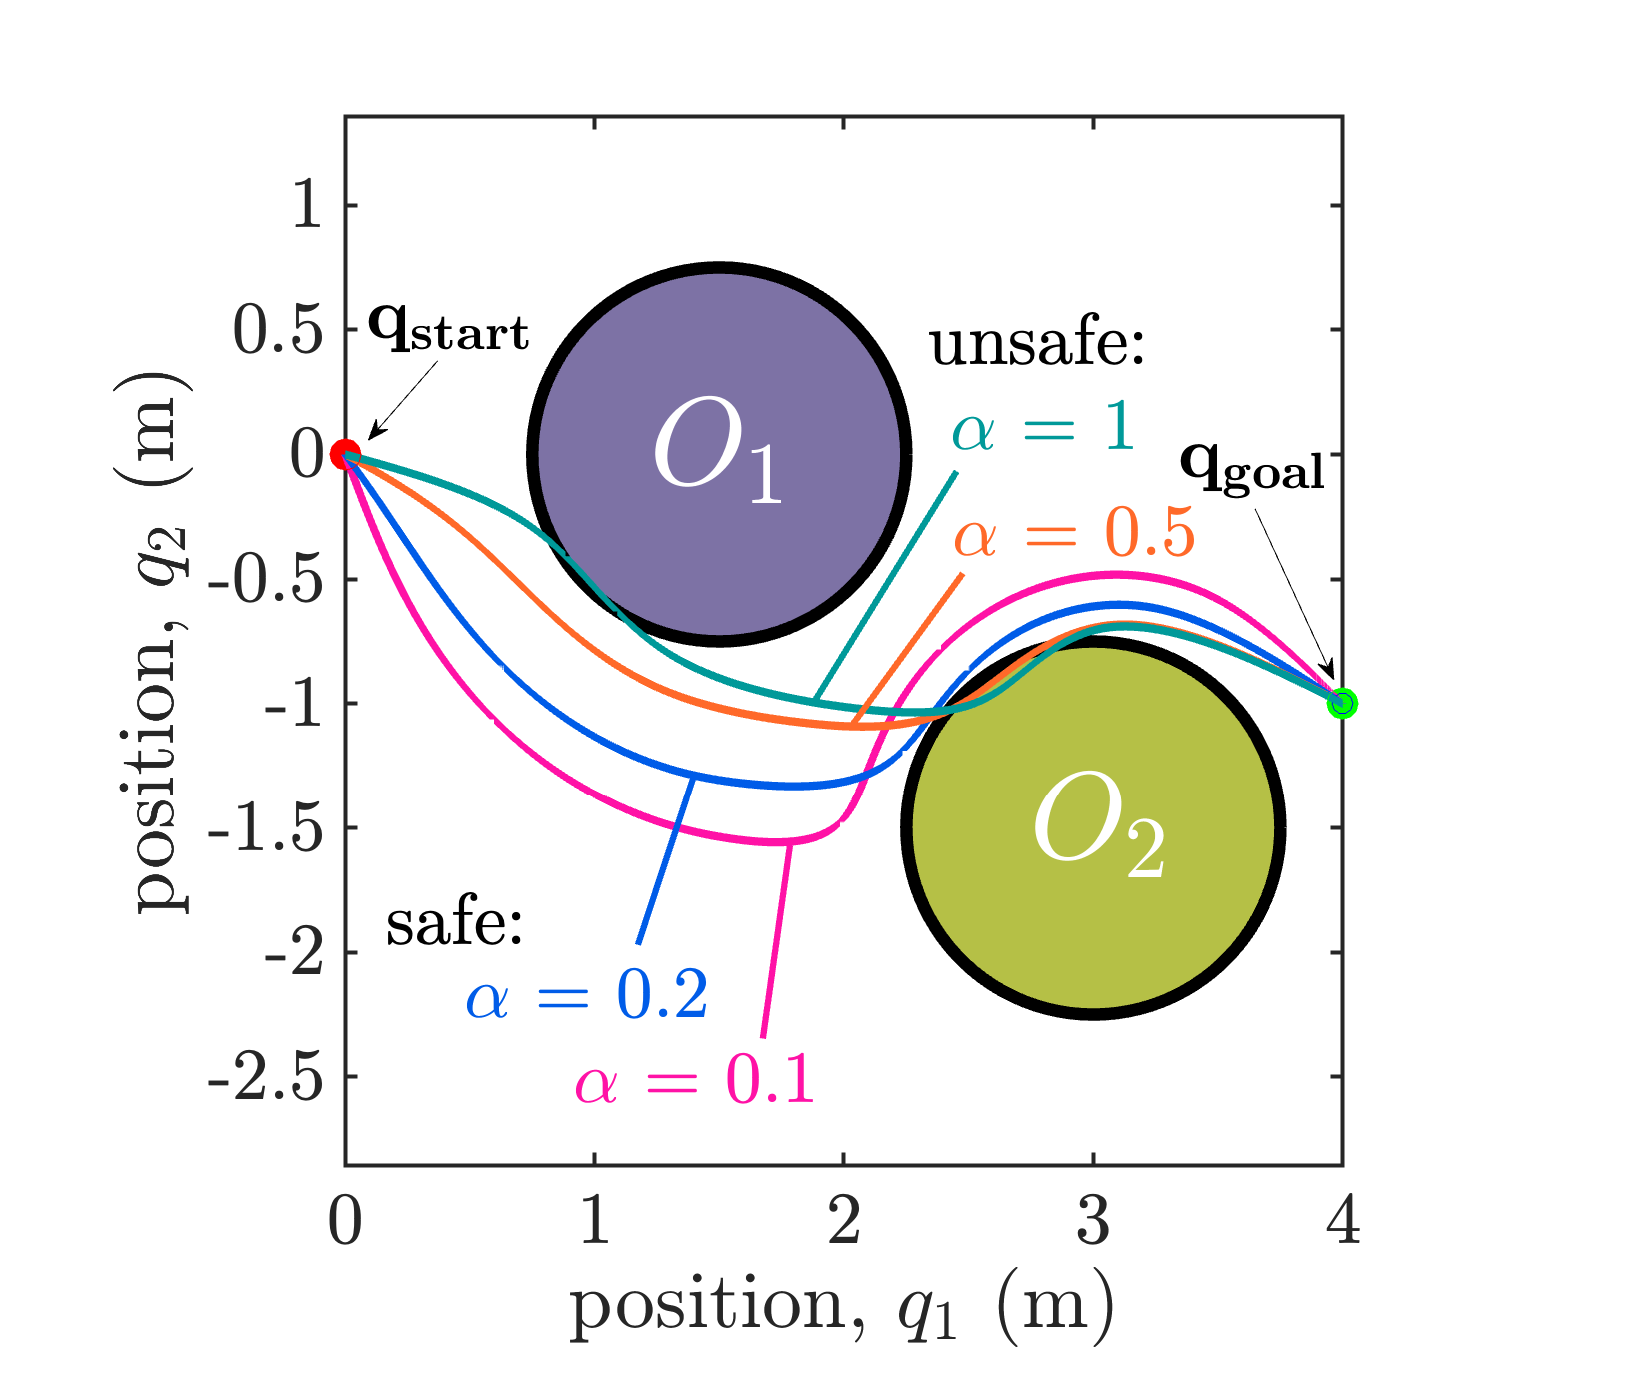
\includegraphics[scale=0.65]{figprint.eps}\\
% \subsection{Unicycle}